\documentclass[11pt,a4paper]{article}
%\usepackage[utf8]{inputenc}
%\usepackage[ascii]{inputenc}
\usepackage[margin=0.7in]{geometry}
%\usepackage{geometry}
\usepackage[dvipsnames]{xcolor}
\usepackage{textcomp}
\usepackage{graphicx}
\usepackage{caption}
\usepackage{subcaption}
\usepackage{amssymb}
\usepackage{amsmath}
\usepackage{tikz}

\begin{document}
\title{Résumé \& Méthodes chapitre V: Filtres numériques}
\maketitle

\section{Définition d'un filtre numérique}
Il existe trois façons de définir un filtre numérique linéaire invariant dans le temps (LIT):
\begin{itemize}
\item : \'Equation aux différences \[ y[n] = x[n] + a y[n-1]\]
\item : Fonction de transfert \[ H(z) = \frac{Y(z)}{X(z)} = \frac{z}{z-a} \]
\item : Réponse impulsionnelle \[ h[n] = a^{n} \]
\end{itemize}
Où $x[n]$ et $y[n]$ correspondent respectivement au signaux discrets d'entrée et de sortie et $X(z)$ et $Y(z)$ à leurs fonctions de transfert.


\subsection{Passage \'Equation aux différences  $\rightarrow$ Fonction de transfert}
On part de l'équation aux différences:

 \[ y[n] = x[n] + a y[n-1]\] 
 
On prend sa transformée en $z$ en appliquant la loi du retard et les propriétés de linéarité:

\[ Y(z) = X(z) + aY(z)z^{-1}   \]

On factorise ensuite de manière à avoir une somme de termes multipliés par $Y(z)$, d'un côté et une somme de termes multipliés par $X(z)$ de l'autre

\[ Y(z)(1 - az^{-1}) = X(z)    \]

On regroupe les termes de façon à faire apparaître d'un côté le rapport $\frac{Y(z)}{X(z)}$ et de l'autre la fonction de transfert

\[ \boxed {H(z) =  \frac{Y(z)}{X(z)} = \frac{1}{1-az^{-1}}}    \]

\subsection{Passage Fonction de transfert $\rightarrow$ \'Equation aux différences}
On prend un autre exemple en partant de la fonction de transfert 

\[ H(z) = \frac{z}{z-1}  \]\\

On réécrit la fonction de transfert pour faire apparaître $Y(z)$ et $X(z)$, les transformées en $z$ des signaux de sortie et d'entrée. Puis on regroupe d'un côté les termes en $Y(z)$ et les termes en $X(z)$ de l'autre

\[ H(z) = \frac{Y(z)}{X(z)} = \frac{z}{z-1} \rightarrow Y(z) (z-1)  =  X(z) z\]

On divise ensuite l'équation par  $z$ pour pouvoir appliquer le théorème du retard de façon direct ($X(z)z^{-1} \rightarrow x[n-1]$)

\[ Y(z) (z-1)  =  X(z) z \rightarrow Y(z) (1-z^{-1})  =  X(z)  \]

On repasse en temporelle en prenant la transformée inverse

\[ Y(z) (1-z^{-1})  =  X(z) \rightarrow y[n] - y[n-1] = x[n]  \]

On exprime alors la sortie courante en focntion des entrées et sorties aux instants précédents

\[ \boxed{ y[n] = x[n] + y[n-1]}  \]

\subsection{Passage \'Equation aux différences/Fonction de transfert $\rightarrow$ Réponse impulsionelle}
On peut obtenir la réponse impulsionnelle en partant de la fonction de transfert ou de l'équation aux différences.\\

Si on part de l'équation aux différences, on remplace $x[n]$ par l'impulsion de Kronecker $\delta [n]$:

\[ y[n] = x[n] + y[n-1] \rightarrow h[n] = \delta [n] + h[n-1] \]\\

Si on part de la fonction de transfert il faut prendre la transformée inverse de la fonction de transfert 

\section{Réponse en fréquence d'un filtre numérique}
\subsection{Défintion} 
La réponseen fréquence d'un filtre numérique fait référence à sa \textbf{Transformée de Fourier}. Pour un signal discret on calcule la transformée de Fourier en partant de la transformée de Fourier et en effectuant le changement de variable suivant:

\[ z =  e^{2 j \pi \nu T_e} \]

Si on reprend une des deux fonctions de transfert précédentes, on obtient : \\

\[\boxed{ H(z) =  \frac{1}{1-az^{-1}}  \rightarrow H(\nu) = \frac{1}{1-ae^{-2 j \pi \nu T_e}}  }\] \\

La fonction de la fréquence $\nu$ ,$H(\nu)$, aussi appelé \textbf{spectre,} ainsi obtenue est généralement complexe ($a +ib$). Pour obtenir de l'information à propos du filtre on regarde donc son module et son argument\\

\newpage
\subsection{Réponse en amplitude}
Soit $H(\nu)$ le spectre fréquentiel d'un système/filtre, alors la \textbf{réponse en amplitude} est donnée par\\

\[ \boxed{|H(\nu)| = \sqrt{\Re(H(\nu))^2 + \Im(H(\nu)) ^2}  }\]\\

avec $\Re(H(\nu))$ la partie réelle du spectre et 
$\Im(H(\nu)$ la partie imaginaire du spectre.\\

Cette fonction indique comment l'amplitude d'une sinusoïde de fréquence $\nu$ va évoluer après le passage de filtre. Si le spectre en amplitude vaut 0 en une fréquence $\nu$ alors une sinusoïde à cette fréquence sera complètement coupé par le filtre. 

\subsection{Réponse en phase}
Soit $H(\nu)$ le spectre fréquentiel d'un système/filtre, alors la \textbf{réponse en phase} est donnée par\\

\[ \boxed{\text{arg}(H(\nu)) = \arctan(\frac{  \Im(H(\nu))}{\Re(H(\nu))})  }\]\\

avec $Re(H(\nu))$ la partie réelle du spectre et 
$\Im(H(\nu)$ la partie imaginaire du spectre.\\

Cette fonction indique le déphasage (décalage temporel) d'une sinusoïde de fréquence $\nu$ entre l'entrée et la sortie du filtre.\\

Cette notion est importante car si le décalage n'évolue pas linéairement avec la fréquence, alors le paquet d'onde se déforme et on obtient de la \textbf{distorsion de phase}

\section{Classification de filtres numériques}
L'analyse de la réponse en fréquence tels que précédemment définie permet de mettre en évidence des catéogries de filtres en fonction de leur réponse en amplitude et en phase.

\subsection{Types de filtres selon leur réponse en amplitude}
\begin{center}
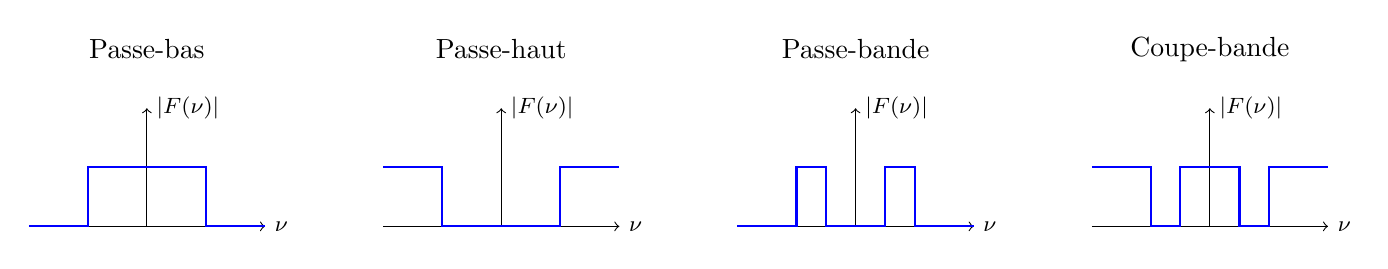
\begin{tikzpicture}
\begin{scope}[scale=1.5]
\draw (0,1.5) [text centered] node{Passe-bas };
\draw[->] (0,0)--(0,1) node[right]{\footnotesize $|F(\nu)|$};
\draw[->] (-1,0)--(1,0) node[right]{ \footnotesize $\nu$};

\draw[thick,blue] (-1,0)--(-0.5,0)--(-0.5,0.5)--(0.5,0.5)--(0.5,0)--(1,0);
\end{scope}

\begin{scope}[scale=1.5,xshift=3cm]
\draw (0,1.5) [text centered] node{Passe-haut };
\draw[->] (0,0)--(0,1) node[right]{\footnotesize $|F(\nu)|$};
\draw[->] (-1,0)--(1,0) node[right]{\footnotesize $\nu$};

\draw[thick,blue] (-1,0.5)--(-0.5,0.5)--(-0.5,0)--(0.5,0)--(0.5,0.5)--(1,0.5);
\end{scope}

\begin{scope}[scale=1.5,xshift=6cm]
\draw (0,1.5) [text centered] node{Passe-bande };
\draw[->] (0,0)--(0,1) node[right]{\footnotesize $|F(\nu)|$};
\draw[->] (-1,0)--(1,0) node[right]{\footnotesize $\nu$};

\draw[thick,blue] (-1,0)--(-0.5,0)--(-0.5,0.5)--(-0.25,0.5)--(-0.25,0)--(0.25,0)--(0.25,0.5)--(0.5,0.5)--(0.5,0)--(1,0);
\end{scope}

\begin{scope}[scale=1.5,xshift=9cm]
\draw (0,1.5) [text centered] node{Coupe-bande };
\draw[->] (0,0)--(0,1) node[right]{\footnotesize $|F(\nu)|$};
\draw[->] (-1,0)--(1,0) node[right]{\footnotesize $\nu$};

\draw[thick,blue] (-1,0.5)--(-0.5,0.5)--(-0.5,0)--(-0.25,0)--(-0.25,0.5)--(0.25,0.5)--(0.25,0)--(0.5,0)--(0.5,0.5)--(1,0.5);
\end{scope}
\end{tikzpicture}
\end{center}

\subsection{Types de filtres selon leur réponse en phase}
Pour ce qui est de la réponse en phase on peut classer les filtres en deux catégories :
\begin{itemize}
\item \textbf{Filtres à phase linéaire}
\item \textbf{Filtres à phase quelconque}
\end{itemize}

Les filtres à phase linéaire évitent la \textbf{distorsion de phase}, c'est-à-dire la déformation du signal liée à une vitesse de propagation qui dépendrait non-linéairement de la fréquence.

\section{Design de filtre}
La réponse en amplitude des filtres décrits au-dessus est parfaite. Il est généralement très compliqué voire impossible d'obtenir une telle réponse en amplitude sur un système réel.\\

La réponse en amplitude d'un filtre réel est généralement sujette à des contraintes et des compromis qu'on peut résumer dans un \textbf{gabarit}. Dans la figure suivante on représente un gabarit pour un filtre passe-bas

\begin{center}
\begin{tikzpicture}
\begin{scope}[scale=1.5]
	\draw[->] (-0.5,0)-- (4,0);
\draw (-0.3,-0.3) node {0};
\draw[->] (0,0)-- (0,3);
\draw (4.1,0.25) node {$f$};
\draw (0,3.5) node {$|H(f)|$};
\draw (1,-0.3) node {$f_1$};
\draw (2,-0.3) node {$f_2$};
\draw (-0.6,1.7) node {$1 - \delta_1$};
\draw (-0.6,2.3) node {$1 + \delta_1$};
\draw (-0.3,0.3) node {$\delta_2$};
\draw (3.5,-0.3) node {$f_e/2$};


\draw[thick,blue](0,1.7)--(1,1.7)--(1,0);
\draw[thick,blue](0,2.3)--(1,2.3)--(1,3);
\draw[thick,blue](2,3)--(2,0.3)--(3.7,0.3);
\end{scope}
\end{tikzpicture}
\end{center}
Avec :
\begin{itemize}
\item $f_e$ la fréquence d'échantillonnage
\item $\delta_1$ : Tolérance en bande passante 
\item$\delta_2$ : Tolérance en bande affiablie  
\item$f_1$ : fréquence de transition-bande passante 
\item $f_2$ : fréquence de transition-bande affaiblie 
\end{itemize}
Ces quantités sont les variables qui guident les choix techniques de la synthèse de filtre. Il va généralement y avoir un compromis entre la largeur de transition $|f_1-f_2|$ et les tolérances en amplitude. Optimiser ces deux variables dans le même temps va généralement impliquer des réalisations de filtres plus complexes.\\

\underline{\textbf{Remarque}}: Le gabarit représenté au-desssus correspond à un filtre numérique. La symétrie en fréquence et la périodisation du spectre implique que toute l'information utile sur le comportement du filtre est contenue entre 0 et $f_e/2$, d'où ce choix de représentation.

\section{Notion de récursivité, pôles et zéros}
Une notion importante relative au design de filtre est celle de la récursivité. Les filtres non-récursifs construisent leurs sorties uniquement à partir d'échantillons du signal d'entrée alors que les filtres récursifs peuvent utiliser les signaux d'entrée et de la sortie pour constituer la sortie à un instant donné.\\
\begin{center}
	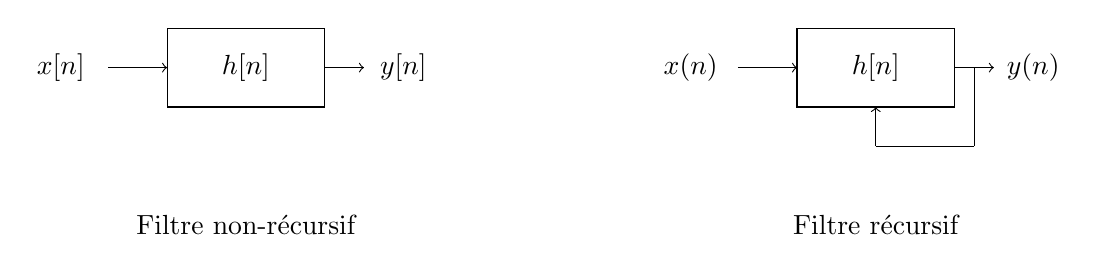
\begin{tikzpicture}
	\draw (2.15,0) node {$x[n]$};
	
	\draw[->] (2.75,0)-- (3.5,0);
	\draw (3.5,-0.5) rectangle(5.5,0.5) ;
	\draw (4.5,0) node {$h[n]$};
	
	\draw[->] (5.5,0)-- (6,0);

	\draw (6.5,0) node {$y[n]$};
	\draw (4.5,-2) node {Filtre non-récursif};
	
	\begin{scope}[xshift=8 cm]
	\draw (2.15,0) node {$x(n)$};

	
	\draw[->] (2.75,0)-- (3.5,0);
	\draw (3.5,-0.5) rectangle(5.5,0.5) ;
	\draw (4.5,0) node {$h[n]$};
	
	\draw[->] (5.5,0)-- (6,0); 
	\draw (6.5,0) node {$y(n)$};

	\draw (4.5,-2) node {Filtre récursif};
	
	\draw[-] (5.75,0)-- (5.75,-1);
	\draw[-] (5.75,-1)-- (4.5,-1);
	\draw[->] (4.5,-1)-- (4.5,-0.5);
	\end{scope}
\end{tikzpicture}
\end{center}

\subsection{Filtres non-récursifs/Filtres à réponse impulsionnelle finie}
Les filtres non-récursifs, aussi appelés filtres à réponse impulsionnelle finie, ont des fonctions de transferts de la forme :

\[ H(z) = 1+ a_1 z + a_2 z^2 + \cdots + a_n z^n  \] \\

Ce type de polynôme en $z$ peut se factoriser en \\
\[  H(z) =  (z-z_1)(z-z_2)...(z-z_n) \]\\

L'ensemble des $z_1 \; ... \; z_n$ est ce qu'on appelle les \textbf{zéros} du filtre. Ce sont des points du domaine fréquentiel où la fonction de transfert s'annule. Les valeurs de l'ensemble des zéros caractérisent le comportement du système.

\subsection{Filtres récursifs/Filtres à réponse impulsionnelle infinie}
Les filtres récursifs, aussi appelés filtres à réponse impulsionnelle infinie, ont des fonctions de transferts de la forme :

\[ H(z) = \frac{1+ a_1 z + a_2 z^2 + \cdots + a_m z^m }{1+ b_1 z + b_2 z^2 + \cdots + b_n z^n}   \] \\

Ce type de polynôme en $z$ peut se factoriser en \\
\[  H(z) =  \frac{(z-z_1)(z-z_2)...(z-z_n)}{(z-p_1)(z-p_2)...(z-p_n)} \]\\

En plus des zéros qui sont définis comme précédemment, une fonction de transfert d'un filtre récursif possède un dénominateur (parce qu'elle fait appel aux entrées précédentes). Les points $p_1 \; ... \; p_n$ de l'espace fréquentiel où ce dénominateur s'annule sont appelés des \textbf{pôles}. Si la fréquence d'excitation d'un sytème s'approche d'un pôle, la fonction de transfert diverge.

\subsection{Filtres non-récursifs vs. Filtres récursifs}
Dans le cadre de ce cours une chose importante à retenir est que les filtres non-récursifs sont les seuls à permettre la réalisation de conditions de phase linéaire.
\end{document}